\documentclass[twoside,11pt]{article} 
\usepackage{amsmath,amsfonts,bm}
\usepackage{hyperref}
\usepackage{amsthm} 
\usepackage{amssymb}
\usepackage{framed,mdframed}
\usepackage{graphicx,color} 
\usepackage{mathrsfs,xcolor} 
\usepackage[all]{xy}
\usepackage{fancybox} 
% \usepackage{CJKutf8}
\usepackage{xeCJK}
\newtheorem{theorem}{定理}
\newtheorem{lemma}{引理}
\newtheorem{corollary}{推论}
\newtheorem{remark}{注}
\newtheorem*{exercise}{习题}
\newtheorem*{example}{例}
\setCJKmainfont[BoldFont=Adobe Heiti Std R]{Adobe Song Std L}
% \usepackage{latexdef}
\def\ZZ{\mathbb{Z}} \topmargin -0.40in \oddsidemargin 0.08in
\evensidemargin 0.08in \marginparwidth 0.00in \marginparsep 0.00in
\textwidth 16cm \textheight 24cm \newcommand{\D}{\displaystyle}
\newcommand{\ds}{\displaystyle} \renewcommand{\ni}{\noindent}
\newcommand{\pa}{\partial} \newcommand{\Om}{\Omega}
\newcommand{\om}{\omega} \newcommand{\sik}{\sum_{i=1}^k}
\newcommand{\vov}{\Vert\omega\Vert} \newcommand{\Umy}{U_{\mu_i,y^i}}
\newcommand{\lamns}{\lambda_n^{^{\scriptstyle\sigma}}}
\newcommand{\chiomn}{\chi_{_{\Omega_n}}}
\newcommand{\ullim}{\underline{\lim}} \newcommand{\bsy}{\boldsymbol}
\newcommand{\mvb}{\mathversion{bold}} \newcommand{\la}{\lambda}
\newcommand{\La}{\Lambda} \newcommand{\va}{\varepsilon}
\newcommand{\be}{\beta} \newcommand{\al}{\alpha}
\newcommand{\dis}{\displaystyle} \newcommand{\R}{{\mathbb R}}
\newcommand{\N}{{\mathbb N}} \newcommand{\cF}{{\mathcal F}}
\newcommand{\gB}{{\mathfrak B}} \newcommand{\eps}{\epsilon}
\renewcommand\refname{参考文献} \def \qed {\hfill \vrule height6pt
  width 6pt depth 0pt} \topmargin -0.40in \oddsidemargin 0.08in
\evensidemargin 0.08in \marginparwidth0.00in \marginparsep 0.00in
\textwidth 15.5cm \textheight 24cm \pagestyle{myheadings}
\markboth{\rm \centerline{}} {\rm \centerline{}}
\begin{document}
\title{\huge{\bf{多项式的唯一析因定理的证明}}} \author{\small{叶卢
    庆\footnote{叶卢庆(1992---),男,杭州师范大学理学院数学与应用数学专业
      本科在读,E-mail:h5411167@gmail.com}}\\{\small{杭州师范大学理学院,浙
      江~杭州~310036}}} \date{}
\maketitle

% ----------------------------------------------------------------------------------------
% ABSTRACT AND KEYWORDS
% ----------------------------------------------------------------------------------------


\textbf{\small{摘要}:}证明了域上多项式的唯一析因定理. \smallskip

\textbf{\small{关键词}:}多项式,唯一析因定理\smallskip


\vspace{30pt} % Some vertical space between the abstract and first section

% ----------------------------------------------------------------------------------------
% ESSAY BODY
% ----------------------------------------------------------------------------------------
\centering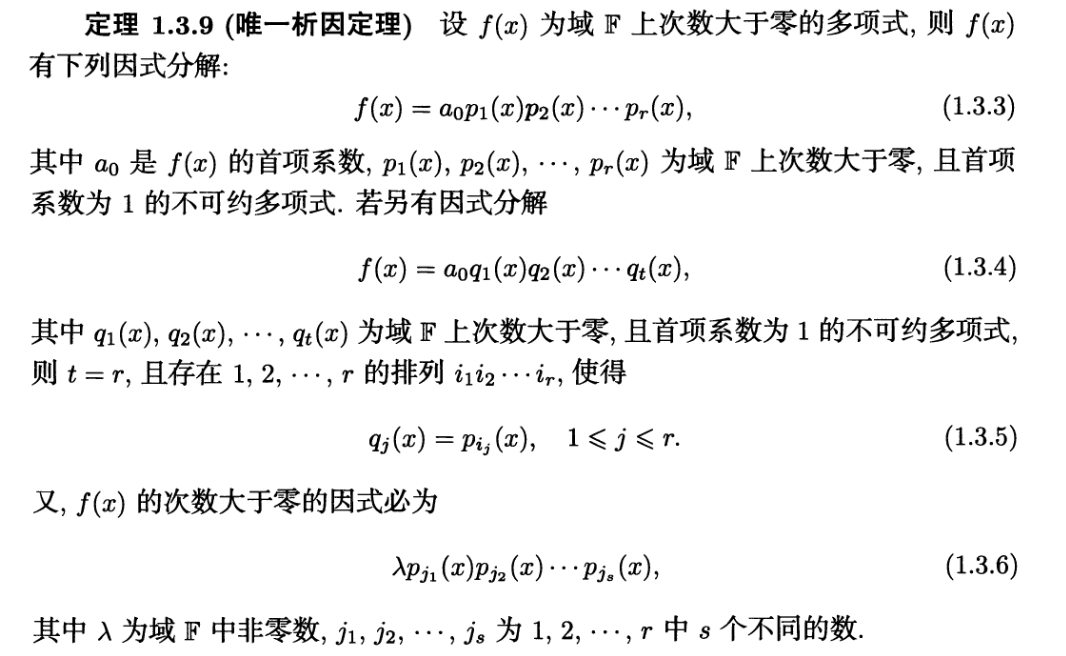
\includegraphics[width=1\textwidth]{/home/luqing/math/higher-algebra-Zhang-Herui/唯一析因定理.png}  
\begin{proof}[\textbf{证明}]
分解的存在性是容易证明的.我只证明分解的唯一性.采用数学归纳法.当$f(x)$
可以分解成$a_0q_1(x)$这种形式时,其中$q_1(x)$不可约,那么容易证明此时分
解是唯一的.假设当$f(x)$可以分解成$a_0q_1(x)q_2(x)\cdots q_n(x)$时,其中
$\forall 0\leq i\leq n$,$q_i(x)$是不可约的,假设此时,分解仍然是唯一的.那
么当$f(x)$能被分解成$a_0q_1(x)q_2(x)\cdots q_n(x)q_{n+1}(x)$时,其中
$\forall 0\leq i\leq n$,$q_i(x)$都是不可约的,我们要证明此时分解仍是唯
一的.这是容易的,因为$$\frac{f(x)}{q_{n+1}(x)}$$能被唯一分解成
$a_0q_1(x)q_2(x)\cdots q_n(x)$(根据归纳假设),而$q_{n+1}(x)$与其它多项
式只有两种关系,要么$q_{n+1}(x)$和其它多项式互质,要么$q_{n+1}(x)$与其它
多项式是常数倍关系.如果是常数倍关系,那么这个常数只能是1,此时能证明$f(x)$的分解$a_0q_1(x)q_2(x)\cdots q_n(x)q_{n+1}(x)$是唯一的.如果是互质关系,是不可能的,这是因为如下的结论:
\begin{lemma}
  $m(x)$为非零多项式,若$p(x)$与$q(x)$互质,则$m(x)p(x)\neq m(x)q(x)$.
\end{lemma}
\end{proof}
\begin{remark}
  数论里的算术基本定理可以类似得证.
\end{remark}

% ----------------------------------------------------------------------------------------
\end{document}








